\section{Approach}
\label{sec:alignmentAlg}
%(mostly along the lines of my presentation for the USCMS workshop because it was time when I was the most active)

%Why align?\\
%How to align?\\
%When align?\\
%How to check that your alignment is good?\\

% DOUBLE CHECK WITH FRANK'S PRESENTATION
% MAKE SURE THERE IS NO PLAGIARISM
The concept of the track-based alignment can be illustrated in the example of the alignment of a toy tracker. When a charged particle passing through a detector (Fig.~\ref{fig:toyTracker_part1}, top left) it crosses a toy tracker which consists of six flat equidistant modules (Fig.~\ref{fig:toyTracker_part1}, top right). If the modules were placed exactly at their designed positions, we would observe the hits exactly at the points where the track crosses modules of ideal geometry (Fig.~\ref{fig:toyTracker_part1}, middle left). However, in reality, the positions and tilts of the modules are different from ones suggested by the ideal geometry (Fig.~\ref{fig:toyTracker_part1}, middle right). Hits, indeed, are recorded at the places where modules are mounted, not at the design ideal places (Fig.~\ref{fig:toyTracker_part1}, bottom left). If we assumed a tracker to be ideal and a track to be smooth, we would see that our hits are off-track (Fig.~\ref{fig:toyTracker_part1}, bottom right). Thus, we recalculate positions of the modules so that all the hits are laying on the same smooth track (Fig.~\ref{fig:toyTracker_part2}, top left). However, these recalculated positions still do not coincide with the actual positions because the modules positions and tilts have more degrees of freedom than the number of hits from one track and also because of uncertainties and possible mismeasurement (Fig.~\ref{fig:toyTracker_part2}, top right). To resolve the ambiguity, we record more and more tracks (Fig.~\ref{fig:toyTracker_part2}, middle left and right). We take into account them all and determine the alignment parameters with necessary precision (Fig.~\ref{fig:toyTracker_part2}, bottom left and right) minimizing residuals between measured and predicted hits.

\begin{figure}[htb]
    \begin{center}
          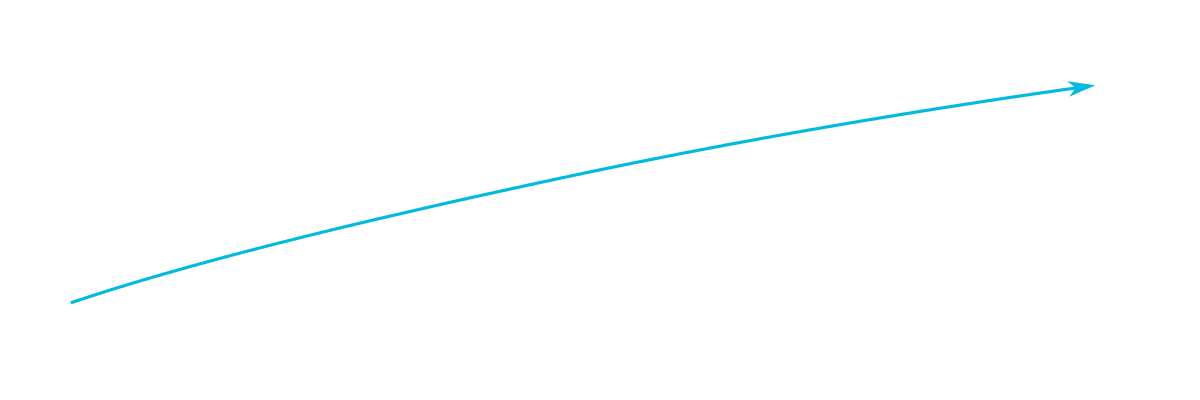
\includegraphics[width=0.45\textwidth]{../figs/Alignment/toyTracker01.png}
          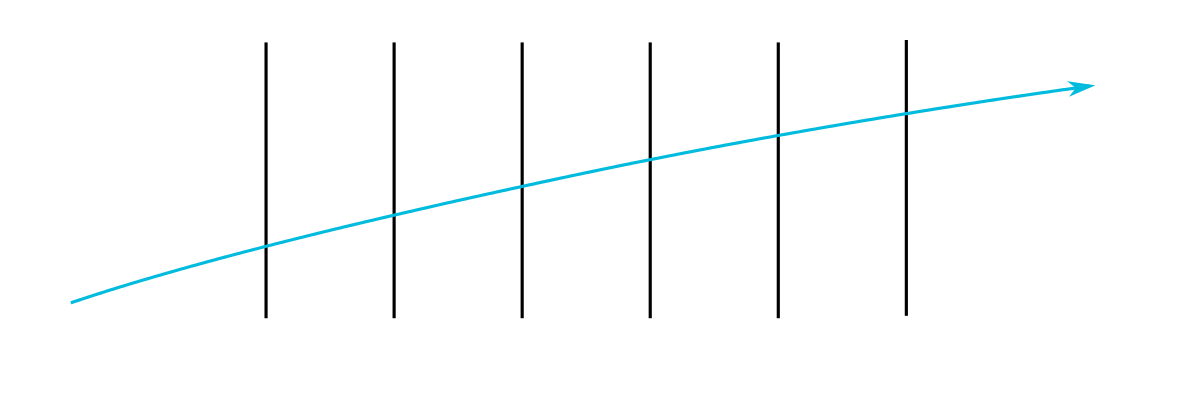
\includegraphics[width=0.45\textwidth]{../figs/Alignment/toyTracker02.png}
        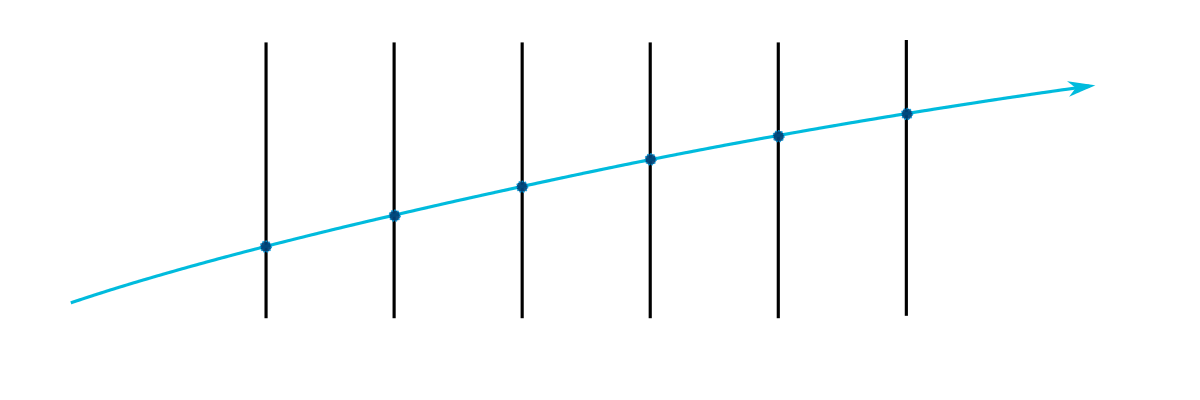
\includegraphics[width=0.45\textwidth]{../figs/Alignment/toyTracker03.png}
        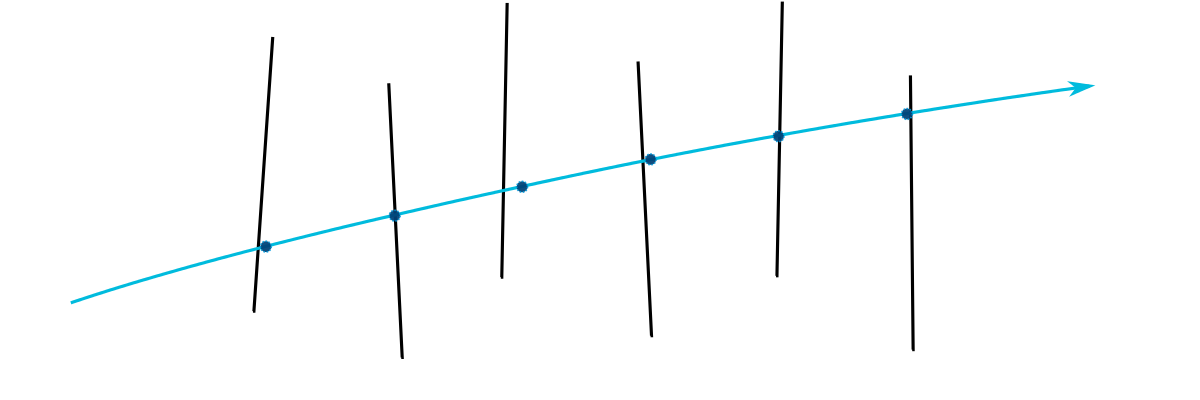
\includegraphics[width=0.45\textwidth]{../figs/Alignment/toyTracker04.png}
        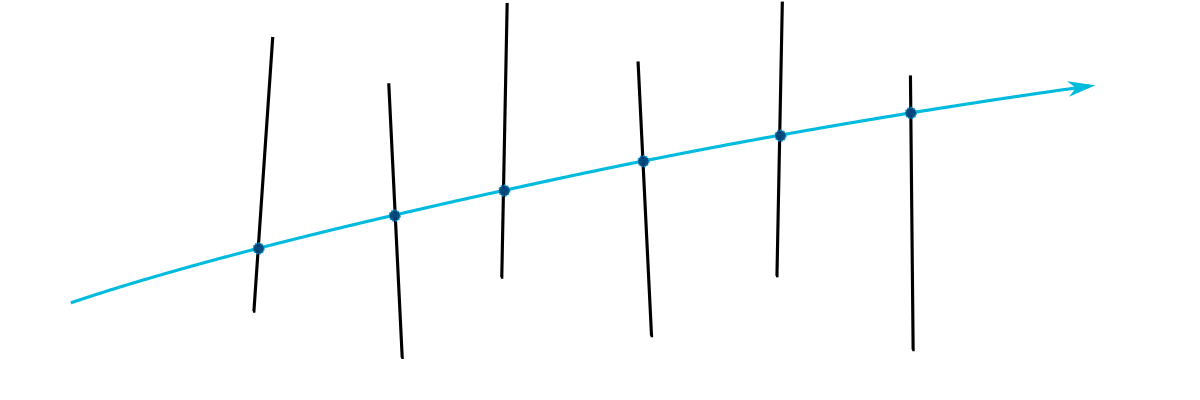
\includegraphics[width=0.45\textwidth]{../figs/Alignment/toyTracker05.png}
        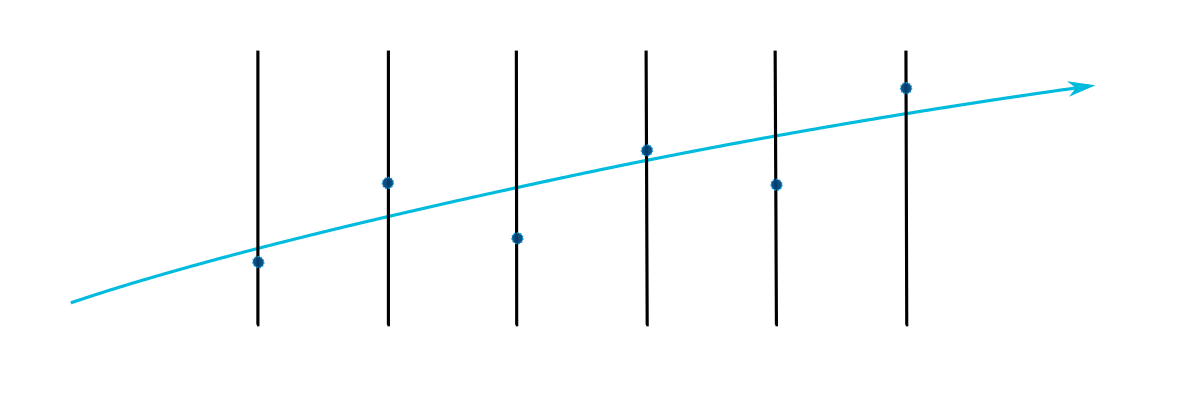
\includegraphics[width=0.45\textwidth]{../figs/Alignment/toyTracker06.png}
    \end{center}
    \caption{The alignment of a toy tracker, part~1~\cite{ref_Frank_presentation}.}
    \label{fig:toyTracker_part1}
\end{figure}

\begin{figure}[htb]
    \begin{center}
        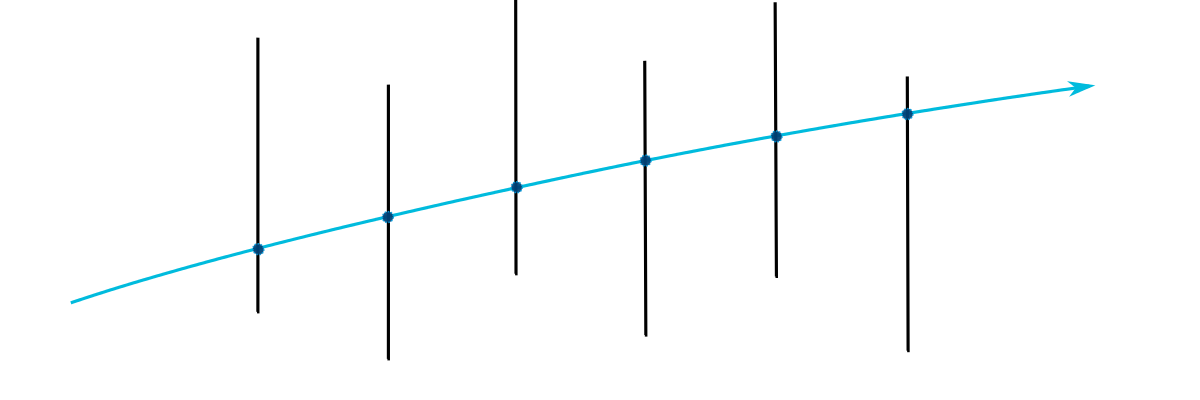
\includegraphics[width=0.45\textwidth]{../figs/Alignment/toyTracker07.png}
        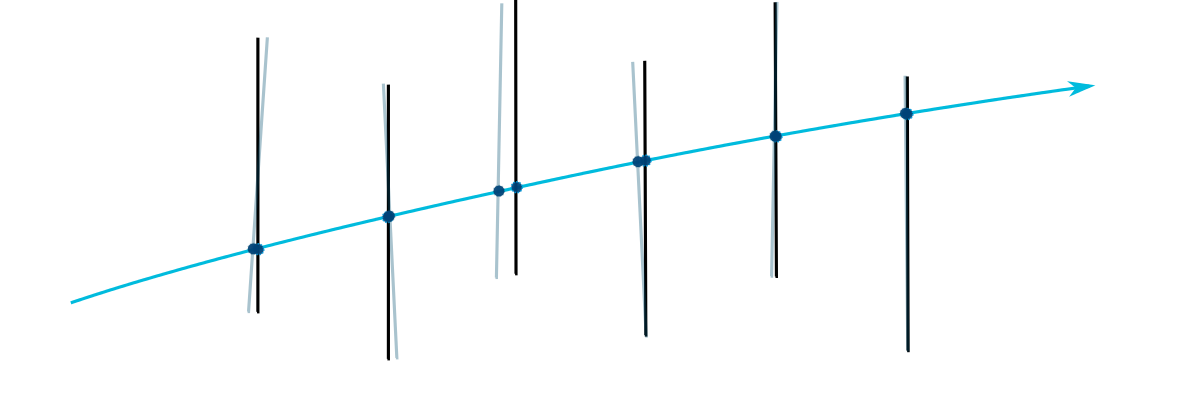
\includegraphics[width=0.45\textwidth]{../figs/Alignment/toyTracker08.png}
        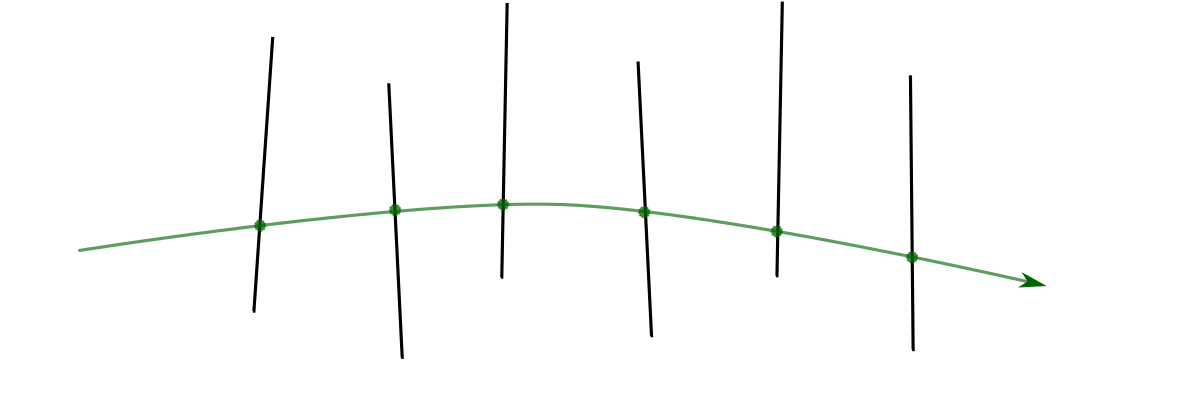
\includegraphics[width=0.45\textwidth]{../figs/Alignment/toyTracker09.png}
        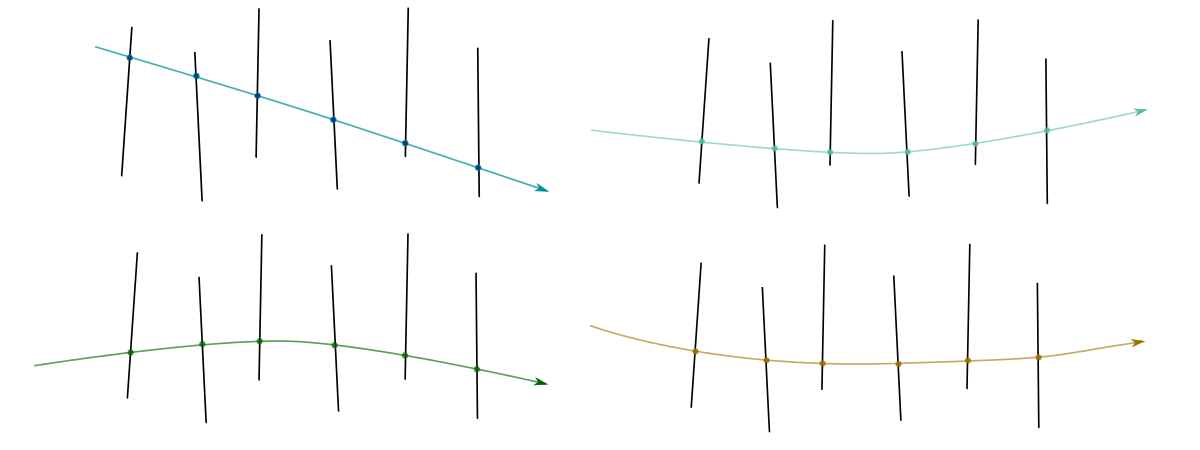
\includegraphics[width=0.45\textwidth]{../figs/Alignment/toyTracker10.png}
        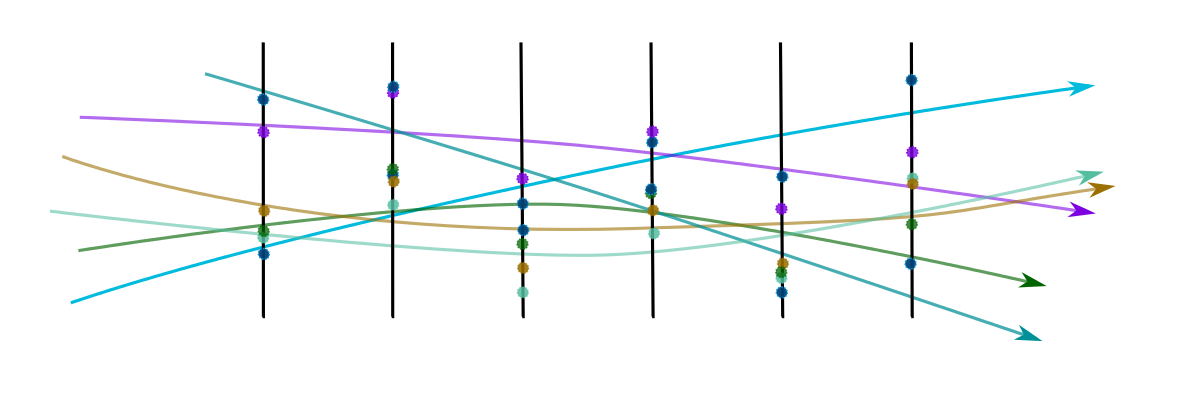
\includegraphics[width=0.45\textwidth]{../figs/Alignment/toyTracker12.png}
        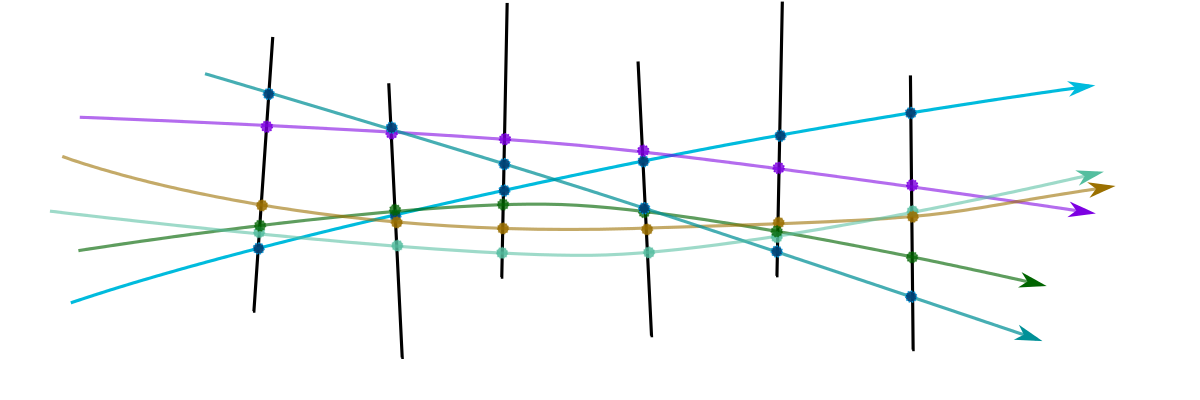
\includegraphics[width=0.45\textwidth]{../figs/Alignment/toyTracker13.png}
    \end{center}
    \caption{The alignment of a toy tracker, part~2~\cite{ref_Frank_presentation}.}
    \label{fig:toyTracker_part2}
\end{figure}

%The CMS tracker contains 1440 silicon pixel modules in PXB and PXF and 15148 silicon strip modules in TIB, TOB, TID, TEC. 

The tracker alignment problem is the least squared problem. The expression to minimize is the following:

\begin{equation}
  \chi^2(\mathbf{p},\mathbf{q})=\sum_j^{tracks} \sum_i^{hits} \left( {\frac{m_{ij}-f_{ij}(\mathbf{p},\mathbf{q_j})}{\sigma_{ij}}} \right)^2
\end{equation}

where $\mathbf{p}$ are parameters describing the tracker geometry, $\mathbf{q}_j$ are parameters of the $j^{th}$ track, $m_{ij}-f_{ij}$ are residuals, distances between the measured hit and a position predicted by the track fit, $\sigma_{ij}$ is the Gaussian error of the measurement.

In CMS, we have two alignment algorithms: Millepede-II~\cite{ref_MPII_Alg} and HIP~\cite{ref_HIP_Alg}. Milledepe-II performs a simultaneous fit of all alignment parameters and all track parameters while HIP performs iterative fits of alignment parameters $\mathbf{p}$ and track parameters $\mathbf{q}_j$.

We can align the large substructures with respect to the global CMS coordinate system and individual modules with respect to the coordinate systems of their substructures. The parameters to align large substructures include three coordinates $X$, $Y$, $Z$ and three angles $\alpha$, $\beta$, $\gamma$. At the module level, we align positions and rotations with respect to the positions and angles of the corresponding large structure (Fig.~\ref{fig:alignmentParameters}). Also at the module level, we align for surface deformations which are described by three parameters per sensor (Fig.~\ref{fig:surfaceDeformations}). 

In addition to particles originating from $pp$ collisions of the LHC, CMS also detects muons that originate from interactions of cosmic particles with the Earth's atmosphere. Tracks left by these two types of particles in the tracking system are referred as collision and cosmic tracks respectively. Both types of tracks are necessary for the alignment. Cosmic tracks pass through the detector vertically and do not allow us to connect different subdetectors to one another. Collision tracks originate from the collision point and go in all directions. However, those tracks which cross TEC are all almost collinear and, therefore, it is difficult to measure $z$-coordinate of TEC modules with collision tracks only.

\begin{figure}[htb]
    \begin{center}
        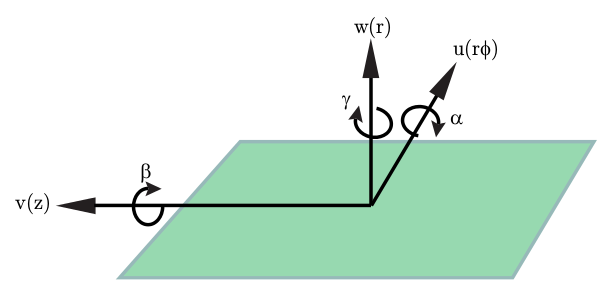
\includegraphics[width=0.70\textwidth]{../figs/Alignment/alignment_strip_coords.png}
    \end{center}
    \caption{Alignment local parameters~\cite{ref_Frank_thesis}.}
    \label{fig:alignmentParameters}
\end{figure}

\begin{figure}[htb]
    \begin{center}
        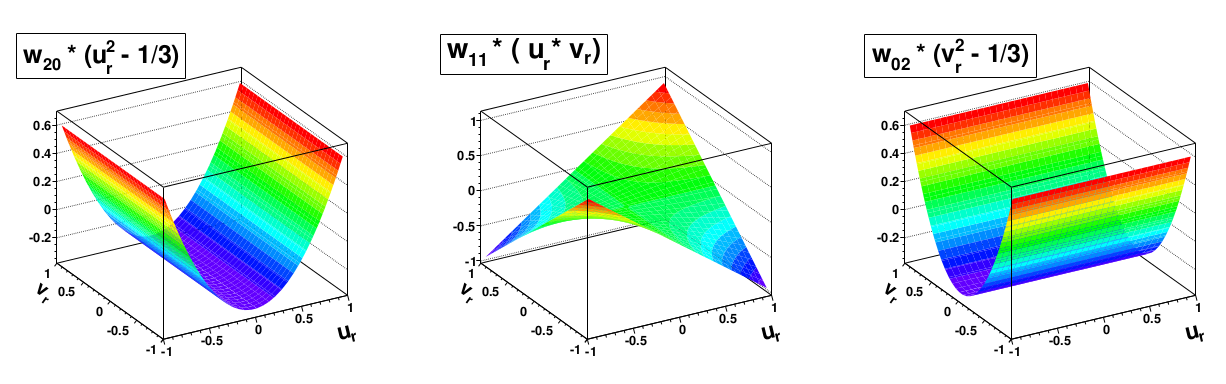
\includegraphics[width=0.90\textwidth]{../figs/Alignment/alignment_surface_deformations.png}
    \end{center}
    \caption{Surface deformations~\cite{ref_Alignment}.}
    \label{fig:surfaceDeformations}
\end{figure}

It is necessary to align a part of the tracking system whenever we suspect a physical change in a location or an orientation this part. First of all, whenever a part of the CMS tracker is taken out and placed back, all large structures are disturbed and, therefore, need to be realigned. Also whenever a magnet is turned on and off, different parts of tracking system shift with respect to one another. Pixel half barrels are not screwed firmly. They are moving along each other on rails and, therefore, need to be realigned every~15 minutes. Realignment on the module level is necessary when modules are replaced. Also, module deformations change when the temperature changes. 

After the procedure of the tracking system alignment is performed, it is necessary to validate the results. Chapter~\ref{sec:alignmentResults} discusses Various tools of alignment validation using the example of the tracking system alignment based on the~2015 data.   

%\begin{figure}[htb]
%    \begin{center}
%        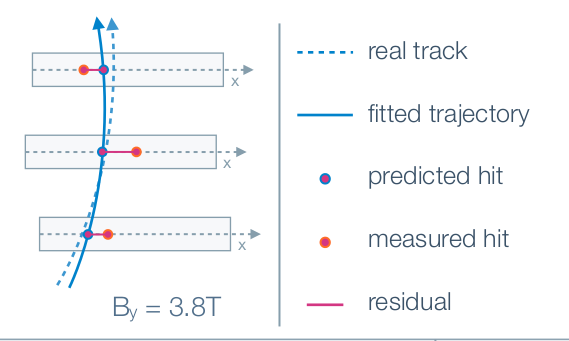
\includegraphics[width=0.70\textwidth]{../figs/Alignment/track.png}
%    \end{center}
%    \caption{Track residuals.}
%    \label{fig:trackAndResiduals}
%\end{figure}

%\begin{figure}[htb]
%  \begin{center}
%    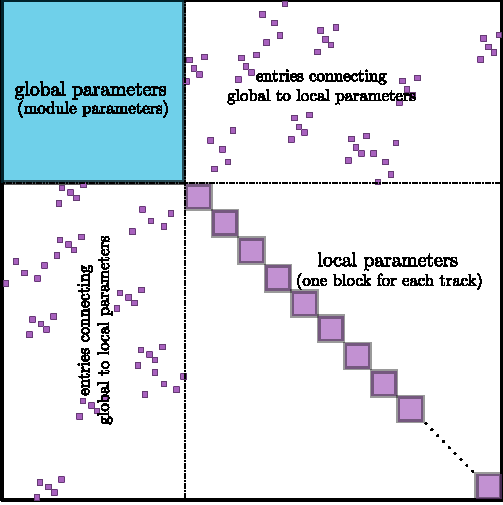
\includegraphics[width=0.70\textwidth]{../figs/Alignment/mpmatrix.pdf}
%  \end{center}
%  \caption{Track residuals.}
%  \label{fig:trackAndResiduals}
%\end{figure}
